%=========================================================================
% sec-future-work
%=========================================================================

\section{On-going Refinements and Improvements}

As we implemented our algorithm and architectural design strategy for the
accelerator, a number of improvements have emerged that point to not only
a speedier validation process but also design of new tools and
methodology to speedup the validation process. First, the level of
abstraction for validation itself can be raised by starting with a
``higher-order'' algorithmic description than coding in Python. In the
case of CNNs, for instance, the networks are described at the highest
level using graphical models. For instance, tensor flow network models
can be used to describe the CNN algorithm that use a dataflow graph where
nodes define tensor flow nodes. Thus a refined strategy would be to use
such tensor flow diagrams and intermediate C++ code can be automatically
generated. Thus, from a given trained model, C++ code can be
automatically generated from the flow graph that is subject to synthesis.

Secondly, the process of conversion from algorithm description in Python
to an architectural description that is input to high-level synthesis is
currently manual. This process can be automated as a refinement of the
original description. CERTUS already provides (and uses) LLVM based
intermediate model that is progressively refined through application of
normal compiler-like transformation. We can treat each such
transformation as a stepwise refinement process and seek to prove their
equivalence to the original source as shown in
Figure~\ref{fig-verification-equivalence}.

%=========================================================================
% fig-verification-equivalence
%=========================================================================

\begin{figure}
  \centering
  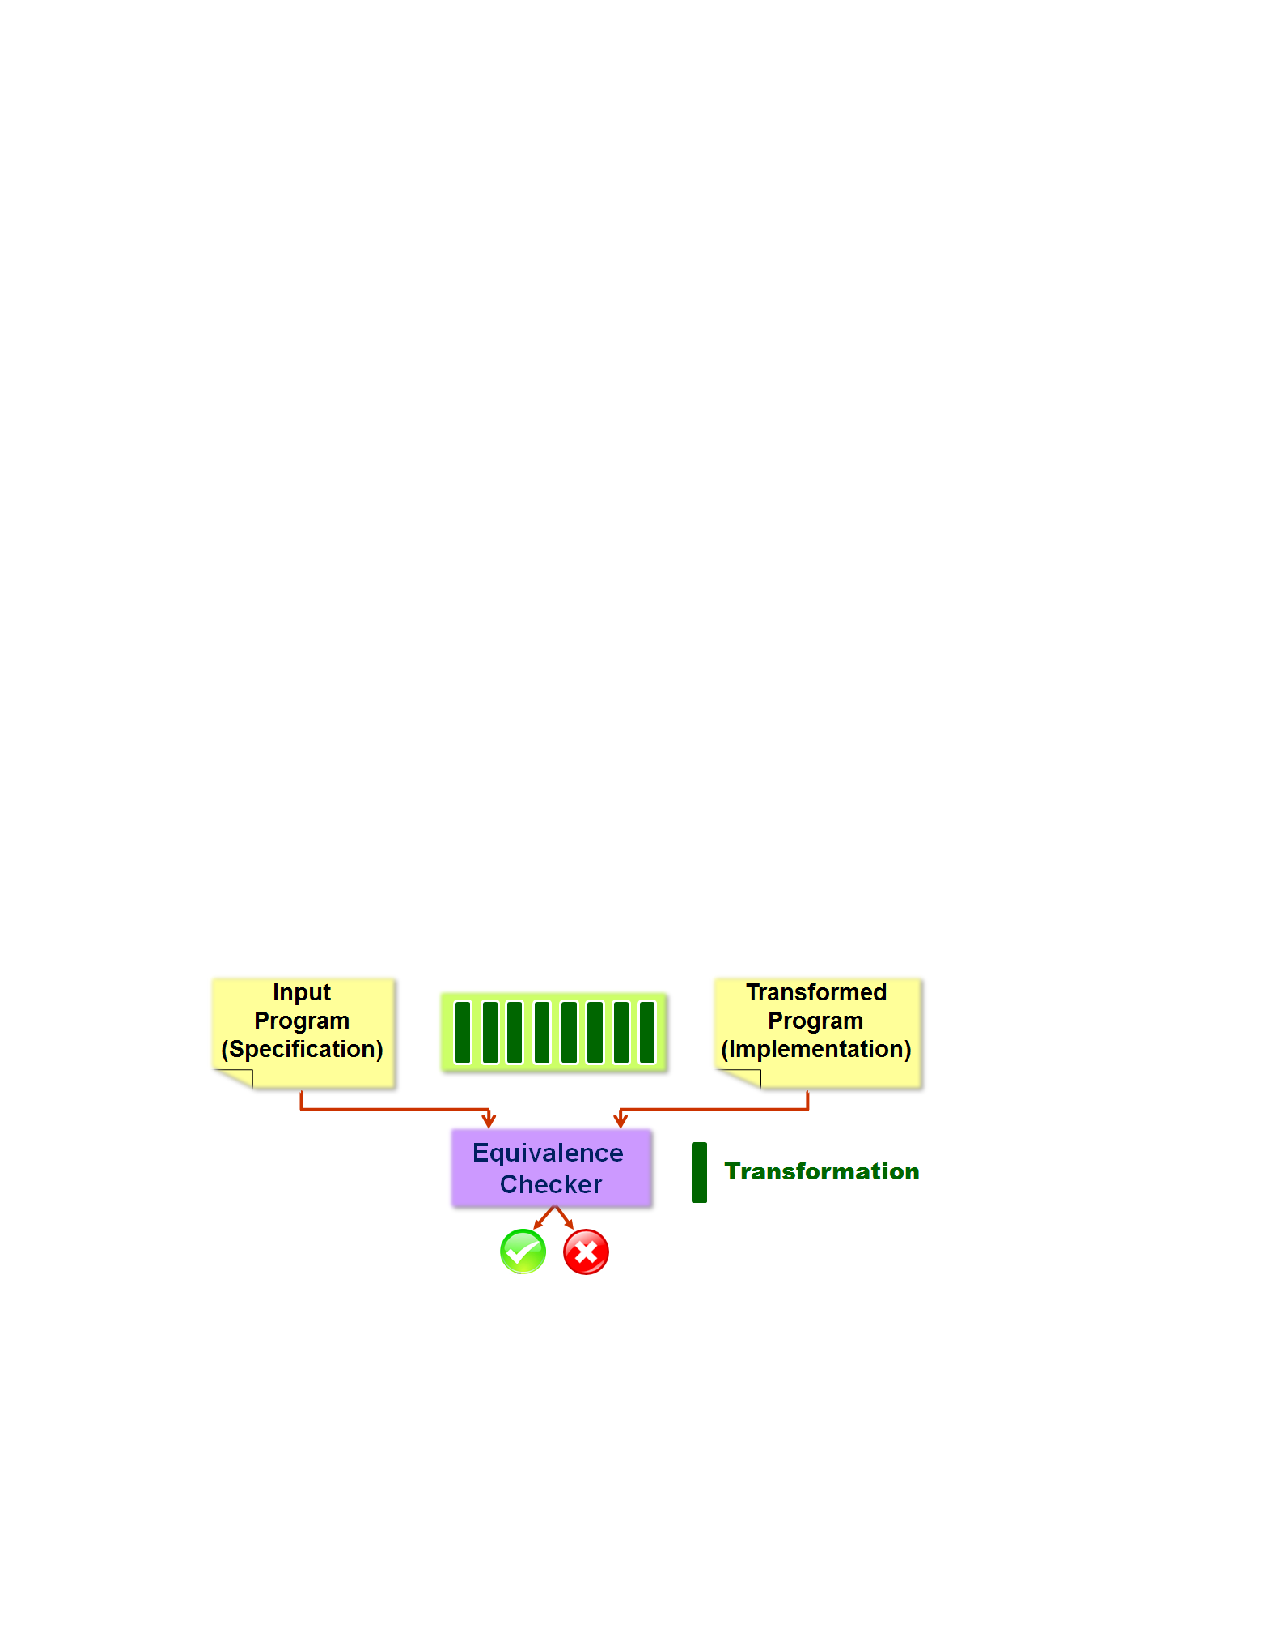
\includegraphics[width=0.7\tw]{verification-equivalence.pdf}
  \caption{\BF{Equivalence Checking Between Input Program and Transformed Program}}
  \label{fig-verification-equivalence}
\end{figure}



The equivalence checks between original and refined description can be
done using model checking on execution traces (execution-based model
checking) or alternatively by building invariant relations at
designer-identified points in the functional behavior that are checked
for equivalence between the source and the refined descriptions.

